\chapter{Background}
\label{chap:back}
\section*{Chapter Outline}
In this chapter we cover the background theory of the various domains which relate to the investigations carried out in this study. We first describe basic theory on the formation, operation, and classification of neuronal cells, how individual cells interconnect to form networks, and how the cells can be characterised using mathematical models. We then describe the theory of network tomography and how it is applied in existing communication networks. Finally, we explain the operation of several classification algorithms and compare their operation.

\section{Neurons and Cortical Circuits}
\label{chap:back:neurons}
% Information on the basics of neuronal cells from the bottom up. Basically a quick overview of everything from molecular communication and synaptic messages to cellular response, morphology etc and onto cortical networks.\\
% Also some information here on LNP models and other ways of characterising neurons.
% \begin{itemize}
%     \item Overview of neuronal cells (intro basically).
%     \item Electrical Characteristics of the signals
%     \item How the electrical signal is "encoded" as electro-chemical processes
%     \item How the electro-chemical process relates to the synapse + cell body
%     \item Describe the e-type differences between cells
%     \item More info on synaptic connections (types, number, neurotransmitters etc)
%     \item Info on m-types of cells. 
%     \item Describe the LNP-cascade model of cell characterisation
%     \item Info on interconnecting cells into a network
%     \item Some info on types of cell networks and how they arrange into layers
%     \item Finish with info on the specific types of above theory that we deal with (layers, mTypes, eTypes, synaptic types and topologies.
% \end{itemize}

A neuron is a type of cell present in the body of most multicellular organisms, differentiated from other biological cells by its ability to be stimulated by an electrical signal, responding in kind with an electrical signal which can be used to excite further neurons. Neurons have multiple roles, with sensory neurons providing sensory input from the organisms environment (light, sound, etc.) and delivering this input to the brain where a different set of neurons form a complex neural network in order to process the sensory input, responding appropriately. Response signals from the neurons of the brain are carried to various parts of the body such as muscles through motor neurons, allowing the organism to physically respond to the environmental sensory input. These different neuronal cells work together to form the nervous system which allow the organism to have contextual awareness of the environment. \par

In this study, we deal solely with the neurons found in the brain; specifically, the neurons investigated are based on prior research into the neurons of the somatosensory cortex of a juvenile rat. This segment is found in the the outer portion of the cerebrum of the brain, referred to as the neocortex. The neocortex is typically treated as being a tightly-packed system of vertical structures (cortical columns), and classified into 6 interconnected horizontal layers. The neurons in this investigation are based on data retrieved from a single cortical column, each classified by layer and a number of other properties discussed later.
\par
While different neurons may have separate roles in the body, the basic form of each neuron is typically made of three sections: the dendrites, the soma, and an axon. An illustration of the layout of a typical neuron is shown in Figure \ref{neuronOverview}. A branched system of dendrites act as an input carrying the electrical signals to the soma (the cell body) which houses the cell nucleus and generates an output signal as some function of the input signals. The output signal is then carried away from the soma by the axon which may then branch, passing the electrical signal onto the dendrites of further cells.\\

\begin{figure}
    \centering
    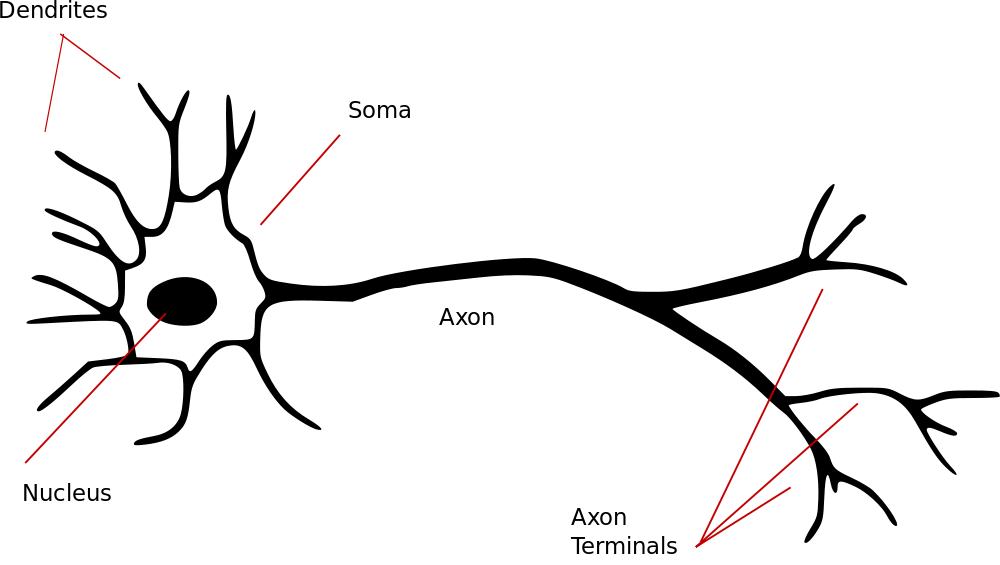
\includegraphics[width=0.75\textwidth]{02-Background/neuron_annotated.png}
    \caption{ Annotated illustration of a typical neuron \cite{neuronAnnotated} showing the branched dendritic tree as input, cell body (soma), and axon as output }
    \label{neuronOverview}
\end{figure}

\par

The axon and subsequent dendrite are generally not directly connected, rather the electrical signal is passed through an electro-chemical interface referred to as a \emph{synapse}. For a given synaptic connection, the neuron acting as a signal source is referred to as the \emph{pre-synaptic cell} while the neuron acting as the signal receiver is referred to as the \emph{post-synaptic cell}. A single pre-synaptic cell may connect to multiple post-synaptic cells, and similarly a post-synaptic cell may receive electrical stimulation from multiple pre-synaptic cells.
\begin{wrapfigure}{R}{0.5\textwidth}
  %  \centering
    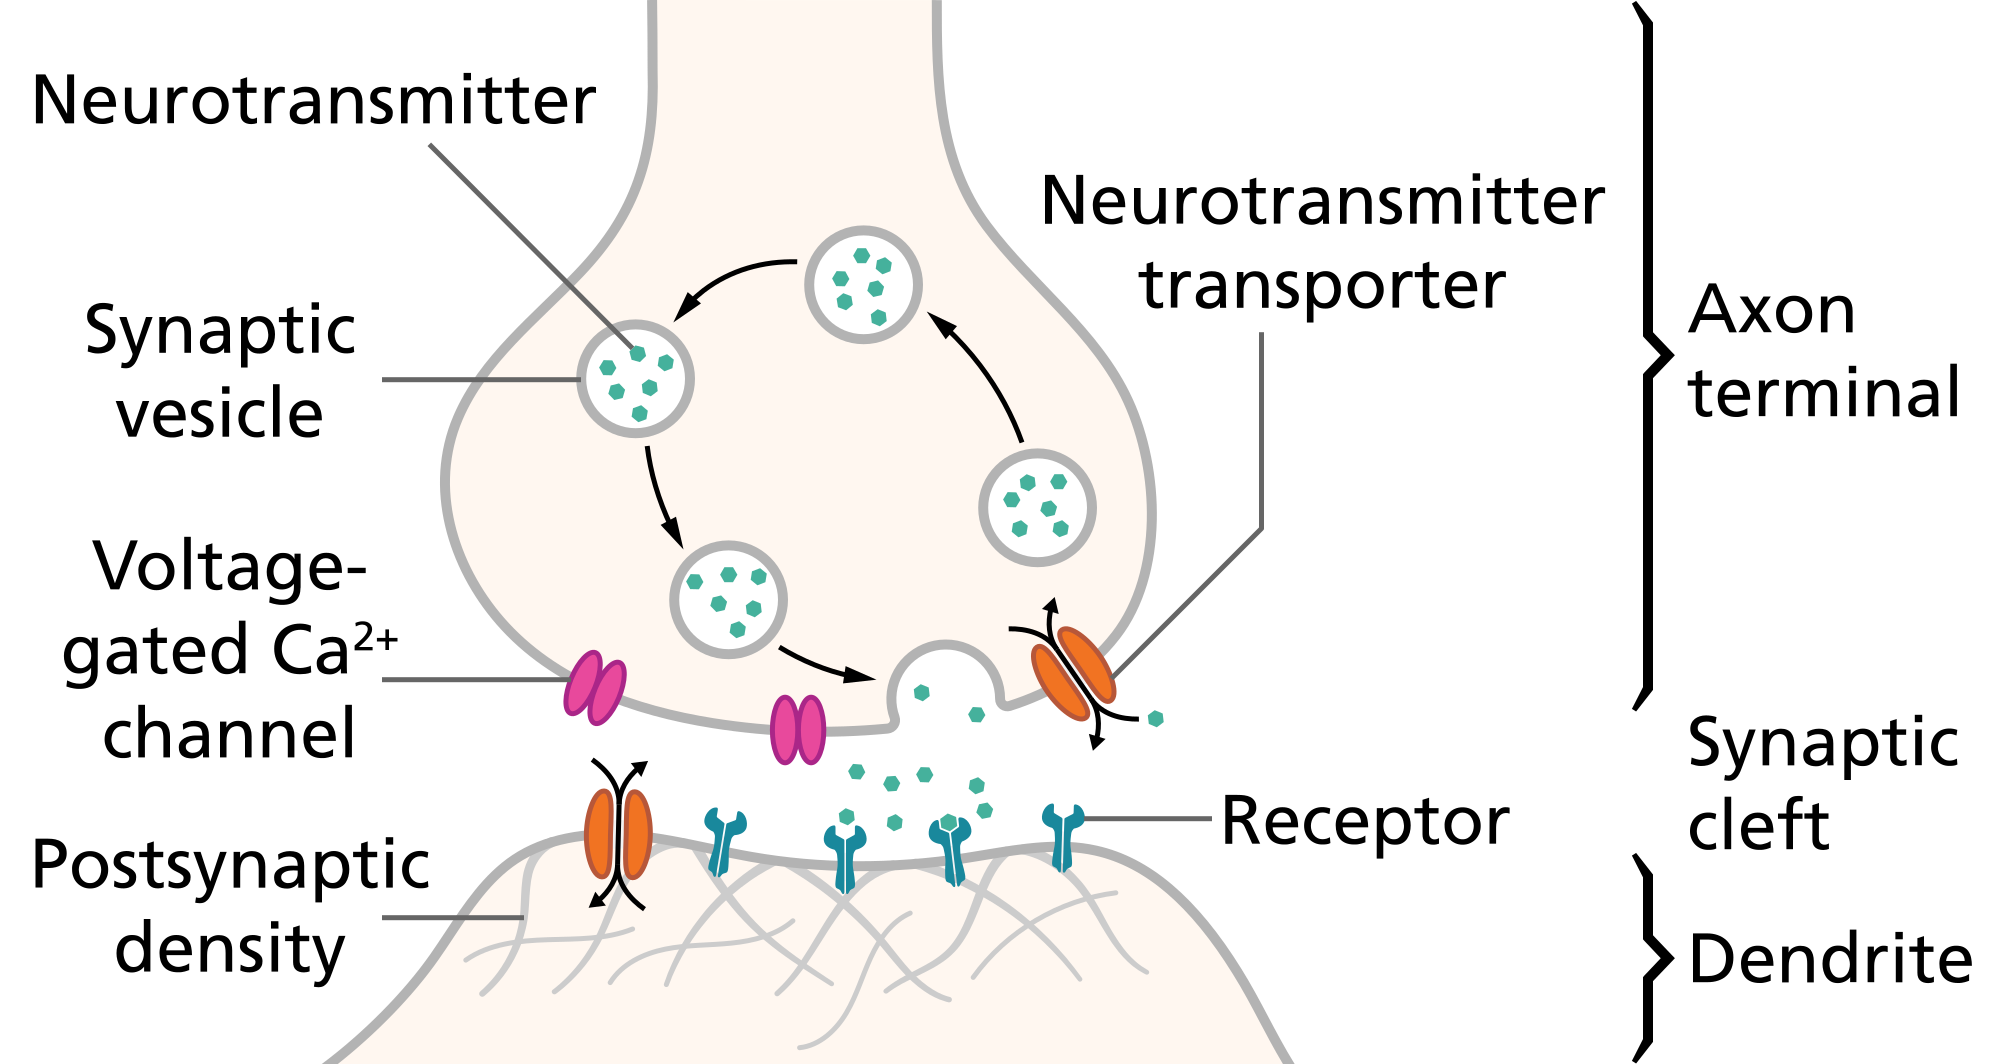
\includegraphics[width=0.5\textwidth]{02-Background/synapse.png}
    \caption{Illustration of synaptic operation \cite{synapseAnnotated} demonstrating the release of neurotransmitters from axon terminal, binding to receptors on opposing dendrite  }
    \label{synapseOverview}
\end{wrapfigure}
As the electrical signal propagates through the axon and arrives at an axon terminal, voltage-gated calcium (Ca\textsuperscript{2+}) channels in the terminal are activated, which causes the release of a \emph{neurotransmitter}, a class of chemical which travels across the synaptic cleft and binds to a receptor at the dendritic receiver. The binding of the neurotransmitter to the receptor elicits some form of response in the post-synaptic cell. The neurotransmitter may cause electrical stimulation in the case of an \emph{excitatory} neurotransmitter, causing a signal to propagate through the dendrite towards the post-synaptic soma, or the neurotransmitter may inhibit the production of an electrical signal in the case of an \emph{inhibitory} neurotransmitter. The neurotransmitter is generally present in the synaptic cleft for a short period of time before it is all bound to receptors, metabolised, or returned to the axon terminal in a process referred to as reuptake.  An illustration of this electro-chemical synaptic process, as well as the general form of a synapse, is shown in Figure \ref{synapseOverview}. The ability for the neuronal system to encode signals (and therefore information) in single molecules such as Ca\textsuperscript{2+} leads to the concept of \emph{molecular communication}, which is the study of this process and how nano-technology may interface with biological components for robust machine-neuron interfaces \cite{mBarrosMolCom}.
\par

While the general form of neurons is consistent, there are a number of properties and classifications used to differentiate between cells to better group them by their input-output response characteristics. In this investigation we classify the individual neurons by neocortical layer, by morphological-type (m-type), and by electrical type (e-type). The m-type of a cell describes its physical properties such as shape, size, and structure. Different m-types exist in different proportions between layers. An overview of the m-types present in the data-set used in this investigation is shown in Figure \ref{mtypeOverview}. The e-type of a cell describes its electrical characteristics which in turn describe how the soma responds to incoming stimulating signals (continuous, burst, delay, etc.). In the neuronal dataset used in this study, the most common e-types are \emph{Continuous Accomodating} (cAC), \emph{Continuous Non-Accomodating}(cNAC), and \emph{Delayed Non-Accomodating}(dNAC), while e-types such as \emph{Continuous Stuttering}(cSTUT) and \emph{Burst Irregular}(bIR) are less common \cite{reconSim}. A complete list of the m-types and e-types in the dataset are tabulated in \ref{tab:m-type_table} and \ref{tab:e-type_table}, respectively.
\begin{figure}
    \centering
    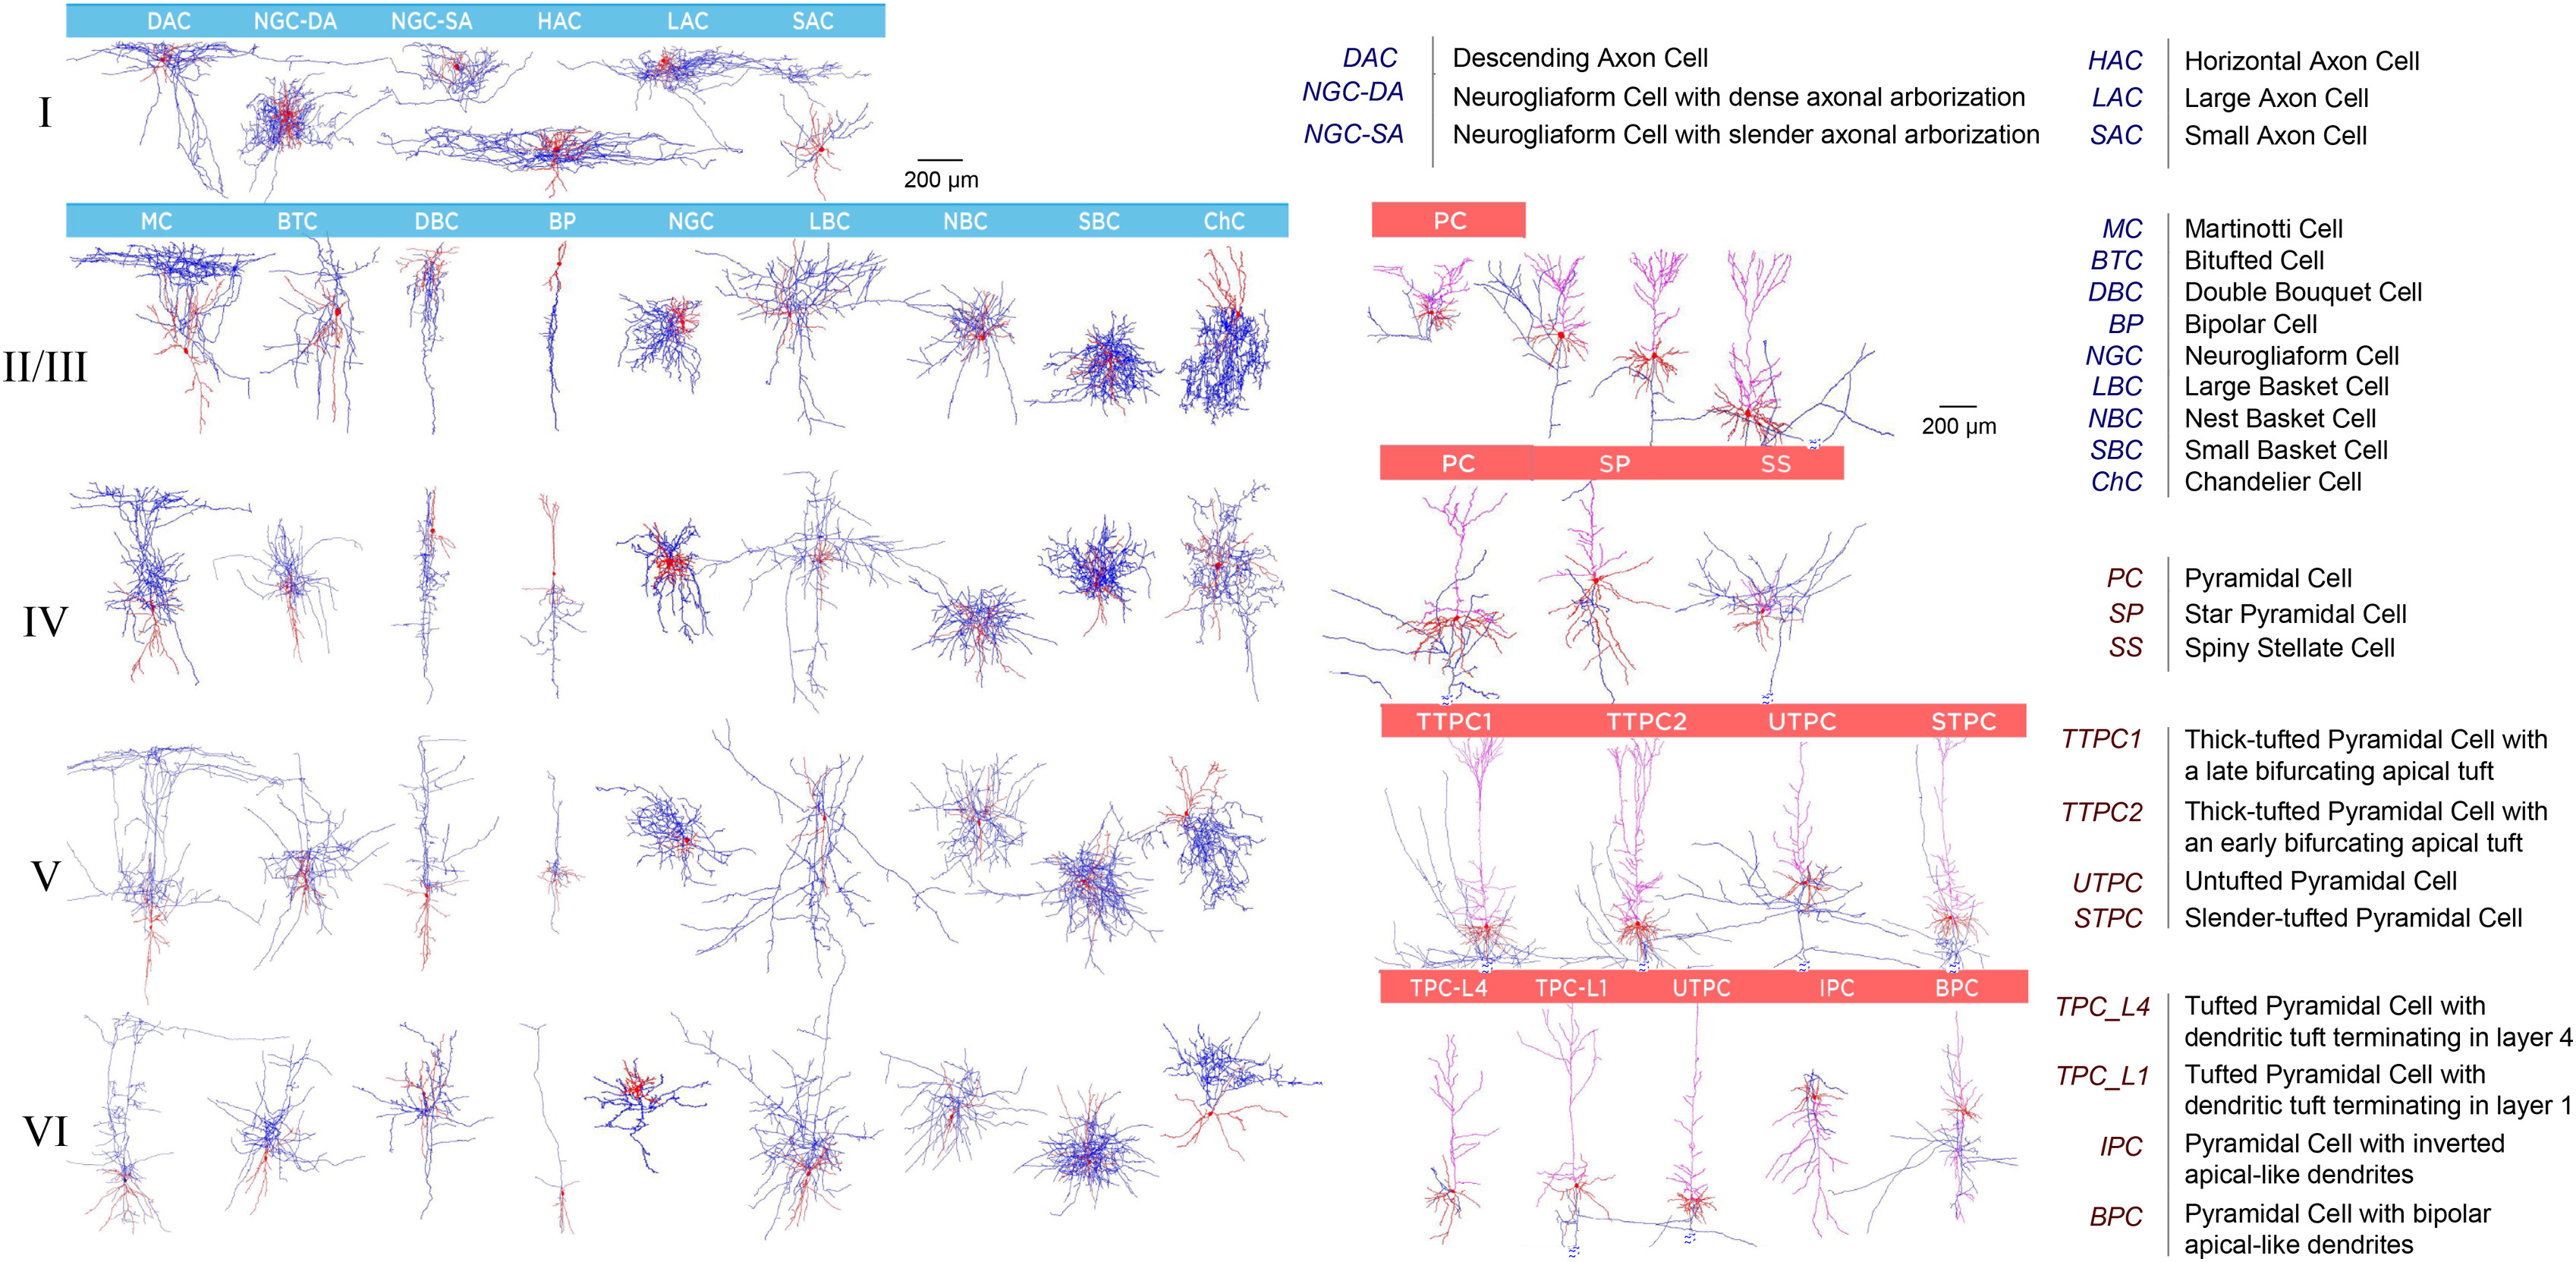
\includegraphics[width=\textwidth]{02-Background/mtypes.jpg}
    \caption{Table of neocortical neuronal morphologies \cite{reconSim} as they appear in each layer. Axons shown as blue, and dendrites as red.}
    \label{mtypeOverview}
\end{figure}

\par

The connection between neurons leads to the emergence of complex neural networks. While the brain as a whole is one large network, there are a number of smaller network topologies that are found across the brain \cite{bbpTop}. These small-world topologies can exist across neocortical layers and they tend to present with similar cell-types. For example, in-hub topologies tend to be formed by excitatory pyramidal cells residing within layers 5 and 6, while out-hub topologies are formed by a mix of inhibitory and excitatory neurons in layers 4 to 6. The "connection probability" between any 2 cells (i.e. the probability of such a connection being observed) is not equal for all cell-pairs. Along with a connection probability, each cell-to-cell pathway has a certain statistical distribution for various connection parameters such as number of synapses in the connection, the type of synaptic connection, cell-separation distance etc. \cite{bbpTop}. These statistical distributions can be used to construct arbitrary network topologies \emph{in silico} and associate a corresponding probability of real-world occurrence. 

\par

Of major interest to us in this investigation is the characterisation of the signals propagated through and between neurons. The response of a neuron is of the \emph{all-or-none} principle; that is, the cell will either respond fully or will not respond at all. The response takes the form of a voltage spike, and the response over time is characterised as a spike train. A sample time-voltage plot from the measurement of the soma-membrane voltage of a simulated neuron is shown in Figure \ref{image:sampleSpike}. As the release of neurotransmitters in the synapse is a response of a spike event rather than of the small variations in resting potential, the response of a post-synaptic cell is therefore also a function of the spike events. Analytically, the spike events are treated in a probabilistic fashion (i.e. the probability of a spike occurring)  to which a Poisson process fits well. The Poisson process describes a model for the estimated time between events, and so when applied in this domain to estimate the time between voltage spikes, the intercellular signals are seen as a \emph{Poisson Spike Train}. This has a number of useful implications for the analysis of these intercellular signals in that the probabilistic modelling of the signal allows for the application of the Poisson model in telecommunicative domains that rely on signal probabilities, such as mutual information and channel capacity. Another implication of this spike-triggered-event property is that the cell can be described as a time-varying process responding to (and with) an impulse train. One such model commonly used is the \emph{Linear-Nonlinear-Poisson cascade}(LNP) model \cite{lnp}.
\par
The LNP model consists of three serial components: a linear filter, a non-linear transform, and a Poisson spike-generating process. This model is typically used to characterise the neurons in the visual system, and so the linear filter is used to describe the response of the neuron in both space and time; typically (in the case of a visual system) the input stimulus is a fixed-size screen and so the space component refers to the pixel-position in space. This filter therefore describes the input image-variation over time that is most likely to elicit a response from the cell. The non-linear transform of the model describes the spike-rate (spikes per second) which is then used in the Poisson-process to generate the spike train. This LNP model is one of many models for the characterisation of the spike-response of a neural cell, however one common property between many of them (and the property of interest in this study) is that of dimensionality reduction. When dealing with the voltage-time measurement of a neuron, the dimensionality of the data increases with every timestep. Through the reduction in dimensionality we can describe the characteristics of an individual cell in a lower, fixed number of dimensions, regardless of the number of datapoints measured. In the LNP model, the dimensionality reduction occurs in the linear-filter component (the non-linearity and Poisson component deal mainly with the production of a spike train which is not required here). While this model generally deals with a spatio-temporal input (i.e. an external screen), we can adapt the concept to use the output spike-train of another neuron as input. As the spike-train is essentially an impulse-train, the resulting linear filter that best characterises the neuron can be estimated as the impulse response of a time varying system taking an impulse train as input and generating a continuous voltage-time output. In this case, a finite-impulse response (FIR) filter model was used. The dimensionality of the model is therefore proportional to the number of filter coefficients in the estimated FIR filter which can be significantly lower than the number of timesteps in the measured data. By measuring the input and output spike trains of a single cell, an estimation can be determined of the k-order FIR filter that best characterises the neuron's impulse response.
\begin{figure}[ht]
    \centering
    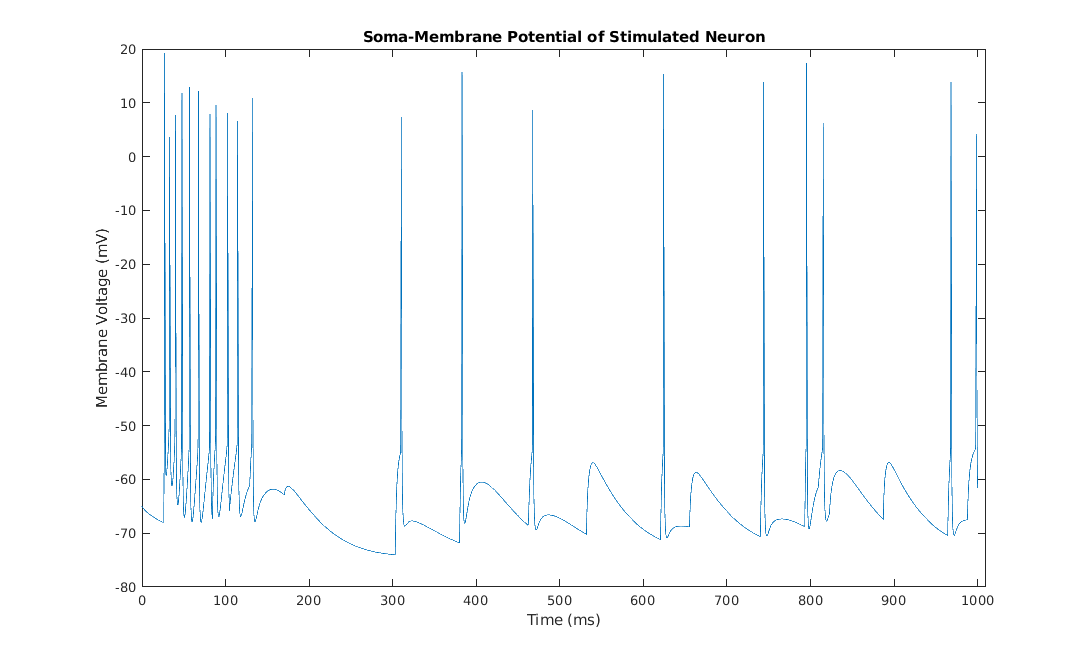
\includegraphics[width=0.75\textwidth]{02-Background/sampleSpikeTrain.png}
    \caption{Spike Train of a Neural Cell}
    \label{image:sampleSpike}
\end{figure}
\par
Previously mentioned was the distinction between excitatory and inhibitory responses. In general, an excitatory neuron is one that increases the spike rate, while an inhibitory neuron is one that decreases the spike rate. This classification is not based on a single cellular property and is instead a result of a number of factors. One such factor is the neuron's e-type. Of the 11 e-types, it was found that only the continuous-adapting (cAD) type was excitatory, while the other types were inhibitory \cite{reconSim}. As well as this, the distinction does not entirely depend on a single cell, but can also refer to the type of synaptic connection between two cells. On the synaptic distinction, the inhibitory/excitatory classification of a given cell is taken from the post-synaptic point of view; that is, if a synaptic connection is inhibitory, then the post-synaptic cell regards the pre-synaptic cell as inhibitory, and vice-versa. This distinction is made more complex by the large number of different synaptic connections (i.e. neurotransmitters/receptors in the synapse). In the dataset used in this study, only 2 synapse-types are provided, differing in receptor/neurotransmitter type. One is inhibitory and is of the GABA class, which responds to the gamma-aminobutyric acid neurotransmitter. The second is excitatory and is made of two neurotransmitter/receptor pairs, one being the N-Methyl-D-aspartate (NMDA) neurotransmitter and the other being the \textalpha-amino-3-hydroxy-5-methyl-4-isoxazolepropionic acid (AMPA) neurotransmitter. \\

\section{Network Tomography}
% Background info from a telecom point of view on the broad scope of network tomography. Discuss different types of tomography (mainly focussing on the types we deal with in the project), as well as how tomography is implemented and used in real-world networks (e.g. internet systems for identifying faults and bottlenecks). Maybe include some of the theory here such as the identifiability of network-level delay using network tomography.
% \begin{itemize}
%     \item Overview of network tomography.
%     \item Describe methods of implementing network tomography (research here)
%     \item Info on how the above methods are used in practice.
%     \item Describe the specific type of network tomography that we use (i.e. basic node-type classification and delay.
% \end{itemize}

Network tomography is a branch of telecommunicative study that deals with the inference of internal network properties from a finite number of endpoint measurements. This concept can be applied in many specific applications, however it is generally used in internet systems to determine link-loss and link-delay characteristics \cite{intTom}. The benefit of this approach is that issues in the network (bottlenecks, broken links etc.) can quickly be identified and located, allowing the service provider to dispatch a small number of engineers to the source of the issue rather than requiring a larger number of engineers across the entire network to manually locate the fault. In these systems, the endpoint data typically comes from measurements at network terminals (e.g. a user's modem) which is then transferred back to the service provider where analysis can be done. Analytically speaking, the problem of broad inference of the entire network can be approximated by describing the measurements as a linear model \cite{intTom} given by:
\begin{equation}
    \label{generalNetTom}
    \vec{y}=\boldsymbol{A}\vec{\theta}+\epsilon
\end{equation}
where $\vec{y}$ is a vector of measurements, $\boldsymbol{A}$ is a routing matrix representing the network node connectivity, $\vec{\theta}$ is a vector of link parameters (delay, loss etc.), and $\epsilon$ is a noise term. The routing network is typically a binary matrix with the $i^{th},j^{th}$ element being 1 to represent a connection between the $i^{th}$ node and the $j^{th}$ node, and 0 representing no connection between the two nodes. The network inference in this case would be estimating the vector $\vec{\theta}$ given some endpoint measurements $\vec{y}$ and knowledge of the networking routing matrix, along with some distribution for the noise parameter $\epsilon$ (Gaussian, Poisson, etc.). For large networks this poses a problem in the computational solution for the linear model, as the dimensionality of $\boldsymbol{A}$ can grow prohibitively large for larger networks. Two options are discussed in \cite{intTom} to solve the linear equation for large networks. One option is to be content with the computational complexity in the linear solution, while the other option is to introduce a regularisation term in order to induce identifiability.
\par
One method of inducing identifiability in link-delay network tomography is through the use of characteristic functions \cite{netTomFour}. The characteristic function of $\vec{y}$ for any I-dimensional $\vec{t}$ is described as
\begin{equation}
    \label{linkDelayCF}
    \phi_{\vec{y}}(\vec{t}) = \prod_{j=1}^{J}\phi_{\vec{\theta_{j}}}(\vec{t}^{T}\boldsymbol{A}^{j})
\end{equation}
where $\phi_{\vec{y}}$ and $\phi_{\vec{\theta_{j}}}$ are the characteristic functions for $\vec{y}$ and $\vec{\theta}$, and $\boldsymbol{A}^{j}$ is the $j^{th}$ column of the routing matrix $\boldsymbol{A}$. The implication of this is that the identifiability problem of the model is satisfied given knowledge of the routing matrix and the characteristic function of the measured data.

\par

There are a number of differences between the networks generally used in network tomography (i.e. internet networks) and the cortical networks investigated in this study. Node-to-node links in internet networks tend to be bi-directional such that information can flow in both directions. This is necessary for the TCP data-link protocol in particular for the acknowledgement of the receipt of packets, along with other uses such as the capability of both uploading and downloading data from some server. In cortical circuits, the cell-to-cell links are mostly unidirectional with signals propagating in a single direction. This has a number of implications for the routing matrix $\boldsymbol{A}$, name that the presence of a 1 for element $\boldsymbol{A}_{i,j}$ implies a high probability of a 0 for element $\boldsymbol{A}_{j,i}$.\\
Another difference between the two classes of networks is the presence of defined routing in internet networks, namely the distinction between \emph{unicast} and \emph{multicast} routing. In unicast routing, the concept is to find some path between any two nodes, passing the signal through other nodes on the path. While any node may have a number of adjacent nodes, the signal is passed along only one of the paths. In multicast routing, the signal is propagated on all outbound paths from the node. This multicast routing principle is most similar to the process of signal propagation in cortical networks. As there is no protocol for specifying specific nodes or endpoints in neural circuits, any signal produced by a cell will be passed to all of its synaptic links with adjacent cells. 

\par

While there exists multiple options for the estimation of the network parameters $\theta$ after inducing identifiability, such as expectation maximisation, maximum likelihood, and maximum a posteriori methods, this study deals mainly with smaller, simpler forms of network tomography. Rather than initially focus on large-scale networks, smaller networks are investigated as a first-step approach to find the features and methods for best characterising the lower-level components of the neuronal networks. As well as this, the design and verification of the network tomography for larger networks increases the computational complexity significantly for the signal processing of the large quantities of produced data, and so is out of the scope of this work.

\section{Information Theory}
\label{chap:back:infTheory}
% Some background details on information theory, up to and including mutual information. Discuss uncertainty and the link between the quality of a network channel and the probability of the events transmitted/received.
% \begin{itemize}
%     \item Overview of what information theory is (analysing information)
%     \item Build up from base to mutual information.
%     \item Describe how mutual information is used to obtain channel capacity
%     \item Describe differences between mutual-information models (i.e. different models representing the same idea based on channel type)
%     \item Mention the type of model we'll be looking at and why (and maybe why it's not a great idea)
% \end{itemize}

Information theory is the study of knowledge, quantising the concept of information into mathematically applicable models. The information theory of discrete systems deals largely with symbols and symbol events. As there is a close link between information theory and probability, a symbol can be thought of being similar to a discrete random variable, where a source may produce a symbol at every event from a set of possible symbol values $\{s_{1}...s_{N}\}$. For an equiprobable set of symbols, the probability of each symbol arising from some event is $1/N$, and the information of a source is given by 
\begin{equation}
    \label{eq:infoSymb}
    I = \log(N)
\end{equation}
where I is the information and n is the number of symbols. Generally, a log to the base 2 is used which gives the information unit as number of \emph{bits} expressed by the source. We can also express the information measure in \ref{eq:infoSymb} as a function of the symbol probability; for an equiprobable set of N symbols, each with probability $P = 1/N$, we can adjust the information equation as
\begin{equation}
    \label{eq:infoEquiProb}
    I = \log(N) = -\log(1/N) = -\log(P) 
\end{equation}
where $P$ is the probability of a given symbol.\\
While this expression is useful for equiprobable systems, it does not adequately represent systems where the probability of each symbol is not equal. For example, consider a source with 2 possible symbols. If the probability of symbol $s_{1} >> s_{2}$, then the observation of some symbol does not cause the observer to gain $log_{2}(2) = 1 bits$ of information as the observer had prior knowledge of the probability of the event. This leads to the definition of a source \emph{uncertainty}, as it is more useful to quantify the source as a measure of how uncertain the observer is of the event value. This uncertainty measure takes the probability distribution of the symbol set into account, and is defined by
\begin{equation}
    \label{eq:uncertProb}
    I(s_{k}) = -\log_{2}(p_{k})
   % H(X) = -\sum_{j=0}^{N}p(x_{j})log_{2}(p(x_{j}))
\end{equation}
where $s_{k}$ is some symbol in the symbol set $\{s_{1}...s_{N}\}$ and $p_{k}$ is the corresponding probability of the corresponding symbol occurring. This measure of information gives the number of bits of information gained as a quanta of information from observing some symbol with a given probability.\\
It is useful to extend this definition of information beyond individual symbols to some measure of the uncertainty of a source generating the events. We can therefore take the expected information gained per symbol on observation of the random variable by taking the sum of information gained from each possible symbol (given by Eq. \ref{eq:uncertProb}), weighted by the probability of observing the symbol. This is given by
\begin{equation}
    \label{eq:entropyDiscr}
    H(X) = -\sum_{k=0}^{N}p(s_{k})\log_{2}(p(s_{k}))
\end{equation}
where H(X) is the expected uncertainty of uncertainty of event source $X$, and $s_{k}$ is some symbol in the set $\{s_{1}...s_{N}\}$. This averaged-uncertainty measure is also referred to as the \emph{entropy} of X, and tells us the average number of bits gained through the observation of the random variable X, or alternatively the average number of bits required to describe X.
\par
Another useful metric in information theory is that of \emph{conditional entropy}, or the entropy of some random variable given the knowledge of another random variable. Given the random variable X, the entropy of X given a particular value of another random variable $Y=y_{k}$ is given by
\begin{equation}
    \label{eq:condEntSing}
    H(X|Y=y_{k}) = -\sum_{j=0}^{N}P(X=x_{j}|Y=y_{k})\log_{2}(P(X=x_{j}|Y=y_{k}))
\end{equation}
Summing over all values of Y and weighting by the probability of the symbol $y_{k}$, we get
\begin{equation}
    \label{eq:condEnt}
    H(X|Y) = \sum_{k=0}^{N}H(X|Y=y_{k})p(y_{k}) = -\sum_{k=0}^{N}\sum_{j=0}^{N}p(x_{j},y_{k})\log_{2}(p(x_{j}|y_{k}))
\end{equation}
where $H(X|Y)$ is the conditional entropy of X given Y, $p(x_{j},y_{k})$ is the joint probability of symbols $x_{j}$ and $y_{k}$, and $p(x_{j}|y_{k})$ is the conditional probability of the same symbols.\\
Given this definition of the conditional entropy, we can obtain an expression for the reduction in entropy of X, given some observed event Y. This is defined by
\begin{equation}
    \label{eq:mutualInf}
    I(X;Y) = H(X) - H(X|Y)
\end{equation}
where I(X;Y) is referred to as the \emph{mutual information} of X and Y. This measurement of mutual information is useful in the analysis of networks as it gives an indication of the amount of information that is transferred between X and Y. In a communication channel, X may be transmitting symbols to Y, and so the mutual information can give a quantitative value to the quality of the link. This leads to the concept of the maximum amount of information that some communication channel can carry, which is defined by
\begin{equation}
    \label{eq:chanCap}
    C = max I(X;Y)
\end{equation}
where C is referred to as the \emph{channel capacity} of the channel linking X and Y.

\par
It is important to note that the expressions for entropy and mutual information given in Eq. \ref{eq:entropyDiscr} and \ref{eq:mutualInf} above are for a \emph{discrete memoryless} system, where a discrete set of symbols can be transmitted at any time, and the observation of a given symbol as some point in time is independent of any previously observed symbols. This is one form of communication channel, however many other forms exist. Applying the same discrete model to a continuous/analogue system by dividing the continuous signal into infinitely small discrete symbols, the equivalent entropy would be infinite. It is clear, therefore, that different models must be defined for different information systems. One such alternate model for analogue channels is given by
\begin{equation}
    \label{eq:chanCapAnalogue}
    C = B\log_{2}\left(1 + \frac{S}{N}\right) bit/s
\end{equation}
where $C$ is channel capacity as before (expressed in this case as bits per second), $B$ is the channel bandwidth in hertz, and $S/N$ is the signal-to-noise power ratio of the transmitted signal. Various other models exist for expressing similar concepts for different communication channels, which are discussed later for specific cases in the form of channels used in this study.

\section{Classification Algorithms}
\label{chap:back:class}
% A short section discussing the classification algorithms used in this project. Talk about what they are, how they're used, and how systems differentiate from each other (i.e. neural net vs SVM vs GMM vs Decision Tree and so on).
% \begin{itemize}
%     \item What is classification
%     \item Non-ML based classification (just probability?)
%     \item Quick desription of machine learning (iterative use of data set to converge on best perf)
%     \item Decision trees/random forest
%     \item GMM
%     \item SVM
%     \item Neural Nets
%     \item Compare the above and maybe talk about what each works best with
% \end{itemize}

Classification is the process of analystically determining which category (or set of categories) that a given set of features belongs to. This is a definition with a rather large scope and classification itself has many variations. For example, classification is a basic trait shared between many organisms; a bird may inspect a number of materials, selecting one based on the classification of which one is most suitable for a nest. In this study, we deal with the computational classification of observations through the use of classification algorithms. Many different classification algorithms exist, each with different traits and suited for different feature sets. These computational classification systems are in use in many applications of everyday life, such as in a vegetable company where damaged or otherwise unmarketable produce can be automatically isolated and removed from the acceptable produce. In general, these classification algorithms are \emph{trained} by collecting a training dataset of observations with a known class, and using this set of data to iteratively adjust the internal coefficients and parameters of the algorithm to best fit the given data. After training, new observations with unknown classes can be passed through the classifier to obtain a "best-guess" estimate of the class that the observation belongs to. In this investigation, we train a number of classification algorithms to determine the neuron cell-type from the observation of the cell's membrane voltage. We compare a number of classifiers to contrast the performance between each, taking into consideration the computational complexity of each.

\par

One such classifier used in this study is a \emph{decision tree}. A decision tree could be best described as a flow-chart generated through training on a dataset to determine observed class. Taking the observation values, it asks a number of binary questions (e.g. is feature 1 > 1.5?) and from either path will determine a class or will ask another binary question. An example of a decision tree is shown in Figure \ref{fig:decisionTreeTitanic} where the classifier predicts whether or not a passenger on the Titanic would survive based on a feature set of their age, sex, and ticket fare. A number of constraints can be set on the training of a decision tree, such as maximum depth, however this form of classifier tends to "overfit", where the model becomes excessively complex/high-order to increase the fit to the training data, which causes the model to perform poorly when classifying on new data.\\
\begin{figure}[ht]
    \centering
    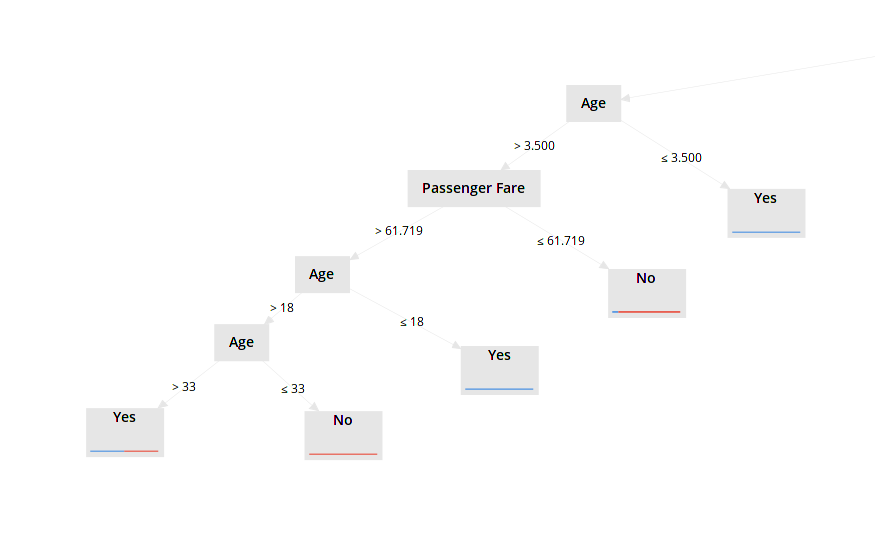
\includegraphics[width=0.75\textwidth]{02-Background/decision_tree.png}
    \caption{Decision tree for classifying survival of the Titanic}
    \label{fig:decisionTreeTitanic}
\end{figure}
One method to overcome the inherent overfitting problem in decision trees is to use a \emph{random forest} classifier. This classifier is constructed as a number of different decision trees and predicting a class based on the mode of the individual tree predictions.

\par

Another form of classifier is based on a \emph{mixture model}, where a number of probabilistic distributions are fit within the feature space. Generally speaking these are multivariate distributions as the feature-space contains more than one dimension. In most applications a Gaussian distribution is used, so this model is referred to as a Gaussian Mixture Model (GMM). The functionality of this system is based on grouping neighbouring observations in the feature-space to produce a number of Gaussian distributions, and based on the proportion of each class in each distribution, a class can be predicted from a given observation based on the distributions into which it fits.

\par
\begin{figure}[ht]
    \centering
    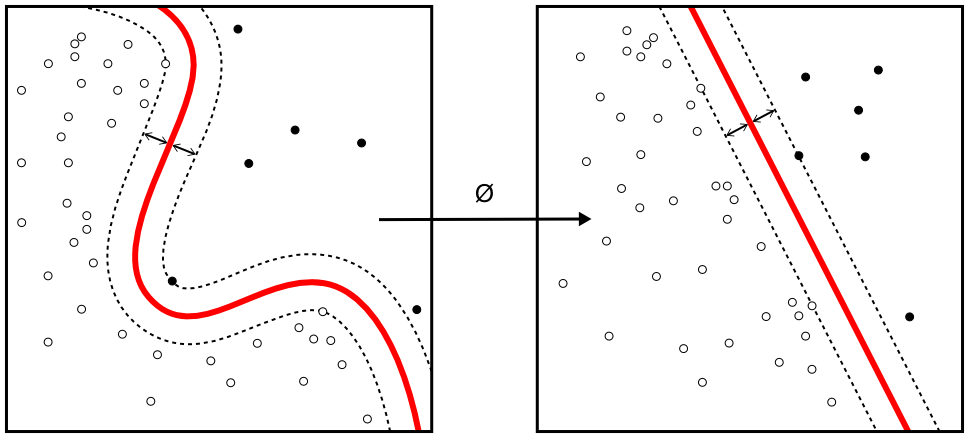
\includegraphics[width=0.75\textwidth]{02-Background/Kernel_Machine.png}
    \caption{Mapping function in a support-vector machine \cite{svmDiagWc}}
    \label{fig:svmMapping}
\end{figure}
A Support-Vector Machine (SVM) is another form of classifier that is commonly used in classification applications. The functionality of an SVM is to determine the hyper-plane that maximises the separation between the classes. A hyperplane is defined as an (N-1)-dimensional plane in an N-dimensional space, such as a line in a 2-D space, or a 2-D plane in a 3-D space. While this is quite similar in principle to logistic regression, the benefit of an SVM is through the use of the \emph{kernel trick}. In order to determine the parameters of the hyperplane, the features must be passed through a \emph{mapping function} which rearranges the features into a higher-order feature space to be separated by such a hyperplane. This mapping function is illustrated in Figure \ref{fig:svmMapping}, where an n-degree polynomial is used to map the features. For complex systems with a large number of features and a high-order mapping function, the resulting feature-space is prohibitively large. The kernel trick is a process used in this case to efficiently find a complex mapping function without explicitly requiring the mapping function to be computed. This allows for a well-performing classifier with a relatively low training complexity.

\par

Neural networks are a form of machine learning models that have recently begun to replace other methods in classification applications. One benefit of a neural network is that through training it can begin to identify and isolate its own features in the observations, allowing for more effective feature extraction in the system with less pre-processing of the data required. The model is made of a layer of input nodes, a layer of output nodes, and a number of "hidden" layers between the two. Each node in the network is a neuron-like unit, taking a number of input values, applying a non-linear \emph{activation function} on the inputs, and producing an output value which is passed to further nodes. In training, the parameters (weights) of these activation functions in each node are adjusted to fit to the training data. Training is done through the comparison of the output of the network with the intended output. The comparison is done through a loss function, which quantises the overall error in the network for the given node-weights. By taking the derivative of the loss function, a gradient can be found at each point in the weight-space for the network which determines the change in weights required for a reduction in the loss. Through iterative steps in the gradient direction for the training data (a process known as \emph{gradient descent}, the model can converge on a points of higher performance. The universal approximation theorem states that a sufficiently large neural network can approximate a continuous function arbitrarily well, which is to say that a neural net should scale well for any classification/regression problem.
